\documentclass[runningheads,a4paper]{llncs}

\usepackage{amssymb}
\setcounter{tocdepth}{3}
\usepackage{graphicx}

\usepackage{array}
\newcolumntype{P}[1]{>{\centering\arraybackslash}p{#1}}
\graphicspath{ {img/} }
\usepackage{graphicx}
\usepackage{boldline}

\usepackage{url}
\urldef{\mailsa}\path|researcher1@example.com, researcher2@example.com, researcher3@example.com|
\newcommand{\keywords}[1]{\par\addvspace\baselineskip
\noindent\keywordname\enspace\ignorespaces#1}

\begin{document}

\mainmatter  % start of an individual contribution

\title{A case study on\\
a new method of carrying a cat}

\titlerunning{A case study on something}

\author{Researcher1 (0000-0000-1111-1111)
\and Researcher2 (0000-0001-1111-2222)\and Researcher3 (0000-0001-2222-1111)}
%
\authorrunning{A case study on something}

\institute{ITMO University, Saint-Petersburg, Russia\\
\mailsa\\
\url{http://www.ifmo.ru}}

\maketitle


\begin{abstract}
  Authors describe results of their ongoing work to research a very important
  problem domain related to something. The paper presents a method and apparatus
  designed to carry a cat.
\keywords{research, data mining, big data}
\end{abstract}


\section{Introduction}

Cat carrying technology field is one of the fastest growing industries today.
Many people use cat carriers to bring their cats outside \cite{item01}.
Cat carrier products that are on the market currently do not meet demanding
requirements of the modern society.

We performed a deep research in cat carrying problem domain and developed a new
very effective technology of carrying a cat.

\section{Related works}

Traditional cat carriers are classified and described in details in
\cite{item01}. Authors of \cite{item02} discuss effectiveness of traditional methods. 

\section{Description of experiment}

A traditional method of carrying a cat is presented on Fig.~\ref{fig:TraditionalCatCarrier}.

%
\begin{figure}
	\centering
	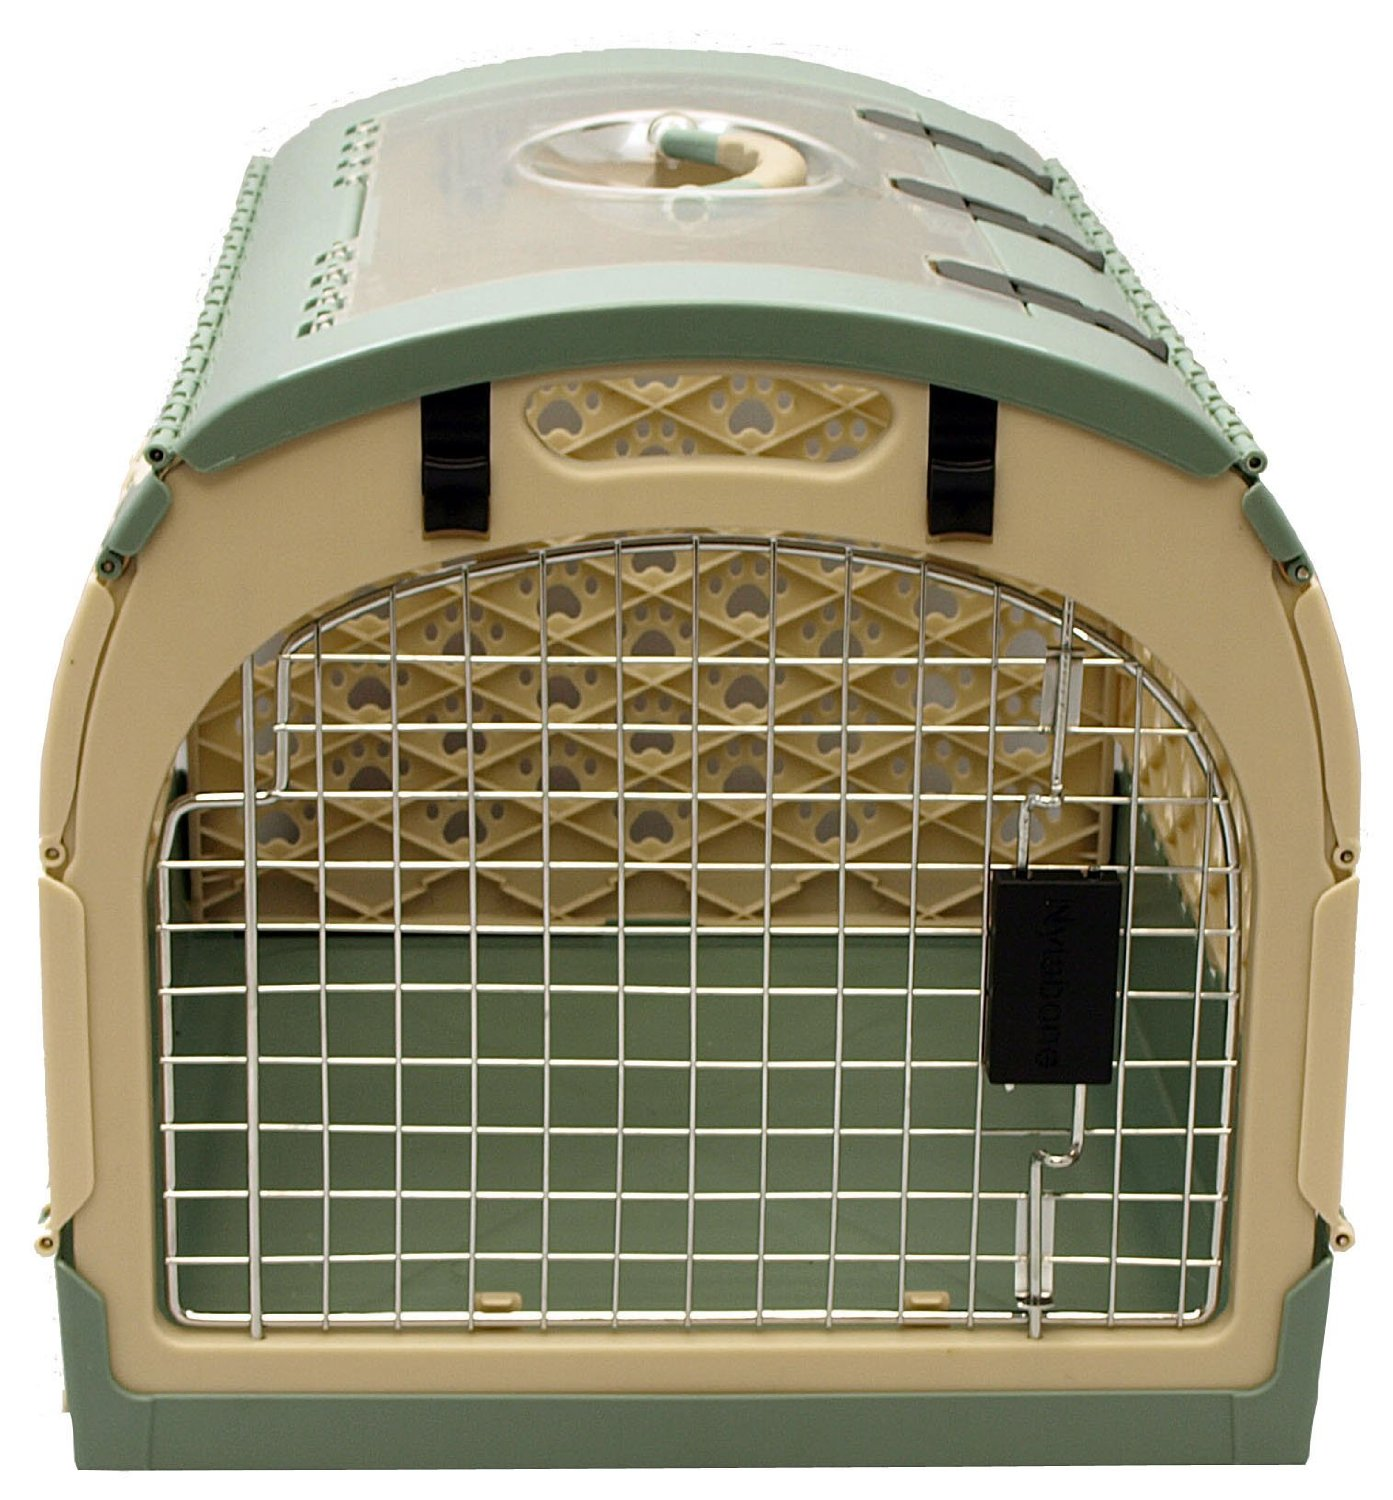
\includegraphics[width=\linewidth]{TraditionalCatCarrier}
	\caption{A traditional cat carrier}
	\label{fig:TraditionalCatCarrier}
\end{figure}
%

The file preparation module is an entry point for a user. The user defines
all necessary environment for subsequent analysis. This environment consists
of a folder with project source code to be analyzed, a set of analyzers
to utilize, a set of excluded analyzer rules and so on.

\section{Tools}

We defined the following set of parameters to compare these frameworks:
popularity among Github \cite{item01} users, CPU and RAM utilization, ability to
parallelize process of analysis and time required to process the same set of projects.

We used a virtual machine with 3Gb of RAM, 3 CPU cores and Ubuntu 14.04
installed as a test host.

\section{Results}

We chose a relatively small sample project (consisted
of roughly 130 files) and configured two plugins in both Coala and Pylama.
Processing time took 112 seconds for Coala and 183 seconds for Pylama.

But it turned out that the most important metric was RAM utilization. We created
a graphical representation of OS memory usage on Fig.~\ref{fig:memusage}.

%
\begin{figure}
	\centering
	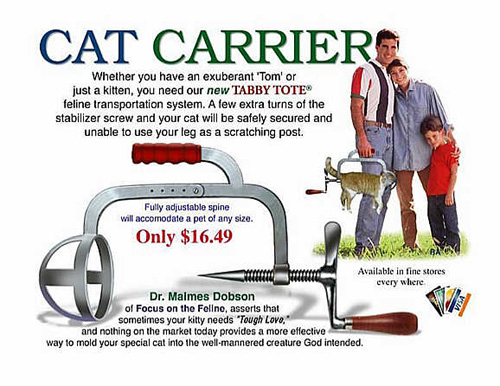
\includegraphics[width=\linewidth]{NewCatCarrier}
	\caption{A proposed cat carrier}
	\label{fig:NewCatCarrier}
\end{figure}
%

Pylama constantly accumulates information about errors so needed RAM grows
almost linearly. This leads to a critical defect that reveals as total RAM
exhaustion. Operating system forcibly terminates Pylama then. Coala does not
accumulate errors and flushes information on errors to stdout periodically, so
the RAM does not exhaust.

Combined comparison results are presented in Table~\ref{tab:compare}. Based on
this results we decided to use Coala as a base framework for future work.
Another possible option is to patch Pylama.

%
\begin{table}
	\caption{\label{tab:compare}Comparison of Coala and Pylama}
	\begin{center}
		\begin{tabular}{p{5cm}|P{2.5cm}|P{2.5cm}}
			\hline
			~                              & Coala & Pylama \\ \hlineB{2}
			Popularity among github users  & +     & -      \\ \hline
			CPU usage                      & +    & +      \\ \hline
			RAM usage                      & +    & -      \\ \hline
			Parallel processing            & +     & -      \\ \hline
			Analysis time (sec)            & 112   & 183      \\ \hline
		\end{tabular}
	\end{center}
\end{table}
%

Next planned step is to process results of analysis by a parsing module
and to standartize them. We are going to store standartized analysis results to
a database. We plan to evaluate a number of relational (e.g. PostgreSQL) and
non-relational databases (e.g. HBase and Cassandra).

\section{Future work}

Authors are going to implement a fully autonomous cat carrying system utilizing
a deep learning algorithm.

We will also try to reduce the weight of our existing solution further. 

\section{Conclusion}

A problem of carrying a cat effectively and in style is actual
at the moment and will become even more actual in the future. There is a huge
demand of cat carrying systems which can work 24*7*365 in hard conditions.

Authors presented an innovative solution and performed field testing. The new
tool is better than existing methods of cat carrying by 146\%.

\begin{thebibliography}{4}

\bibitem{item01} Researcher5, R.R.: Problems of carrying a cat. J. Nature. 1 (200), (2010)

\bibitem{item02} Researcher6 R. et al.: Carrying a cat
  effectively. In: Proceedings of the Nth international
  conference on Cat Carrying, pp. 200--210. Cat Carriers Society (2011)

\bibitem{item03} Researcher7, R.R.: Introduction to carrying a cat. NN
  Publishing, New York (2008)
  
\bibitem{item04} Google, \url{https://google.com}

\end{thebibliography}

\end{document}
